\begin{figure}[H]
  \begin{center}
    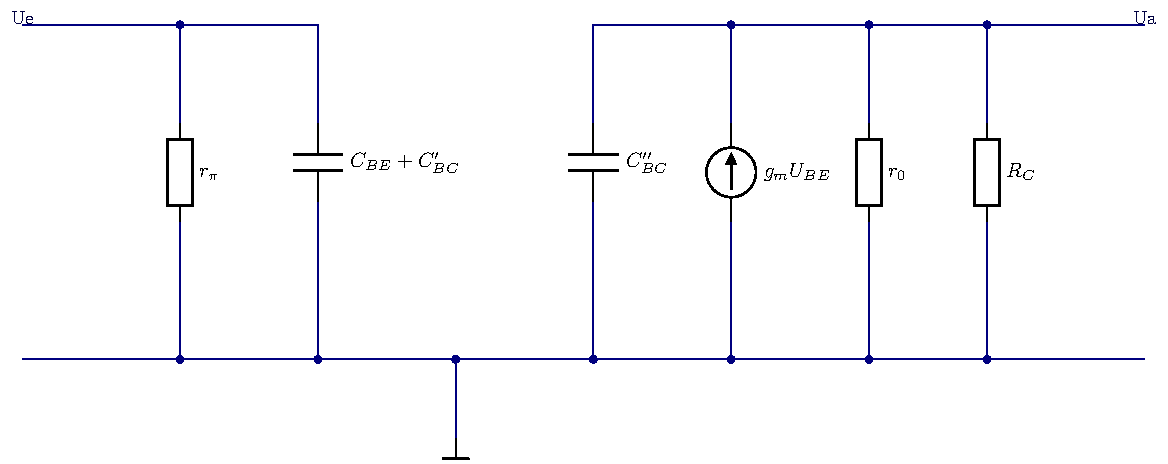
\includegraphics[width=0.618\textwidth]{circuits/commonEmitter_freq.pdf}
  \end{center}
  \caption{ESB der Emitterschaltung mit Millerkapazitäten}
\end{figure}

Die obere Grenzfrequenz der Schaltung wird durch die parasitären Kapazitäten des
Bipolartransistors bestimmt, die untere durch die Koppelkondensatoren der Schaltung

Eingangskreis:
\[0 = \frac{U_1}{r_\pi} + U_1 j \omega (C'_{BC}+C_{BE})-I_b\]

\noindent Ausgangskreis:
\[0 = g_m U_1 + \frac{U_a}{r_0 // R_C} - U_a j \omega C_{BC}''\]

\noindent Übertragungsfunktion
\[\frac{U_a}{U_e} = \frac{\frac{1}{r_\pi} +
    j\omega(C_{BC}'+C_{BE}) -g_m}{\frac{1}{r_0 // R_C} - j\omega C_{BC}''}\]

\noindent Grenzfrequenz
\[\omega_{gr} = \frac{1}{(C_{BE}+C_{BC}')r_\pi }\]

\[\left( \omega_{gr} = \frac{1}{(C_{BC}' + C_{BE})\cdot \frac{1}{g_m} - r_0
      C_{BC}''} \right) ? \]